%
\begin{isabellebody}%
\def\isabellecontext{Examples{\isadigit{3}}}%
%
\isadelimtheory
\isanewline
\isanewline
%
\endisadelimtheory
%
\isatagtheory
\isacommand{theory}\isamarkupfalse%
\ Examples{\isadigit{3}}\isanewline
\isakeyword{imports}\ Examples\isanewline
\isakeyword{begin}%
\endisatagtheory
{\isafoldtheory}%
%
\isadelimtheory
%
\endisadelimtheory
%
\isamarkupsubsection{Third Version: Local Interpretation%
}
\isamarkuptrue%
%
\begin{isamarkuptext}%
In the above example, the fact that \isa{{\isasymle}} is a partial
  order for the natural numbers was used in the proof of the
  second goal.  In general, proofs of the equations may involve
  theorems implied by the fact the assumptions of the instantiated
  locale hold for the instantiating structure.  If these theorems have
  been shown abstractly in the locale they can be made available
  conveniently in the context through an auxiliary local interpretation (keyword
  \isakeyword{interpret}).  This interpretation is inside the proof of the global
  interpretation.  The third revision of the example illustrates this.%
\end{isamarkuptext}%
\isamarkuptrue%
%
\isadelimvisible
%
\endisadelimvisible
%
\isatagvisible
\isacommand{interpretation}\isamarkupfalse%
\ nat{\isacharcolon}\ partial{\isacharunderscore}order\ {\isachardoublequoteopen}op\ {\isasymle}\ {\isacharcolon}{\isacharcolon}\ nat\ {\isasymRightarrow}\ nat\ {\isasymRightarrow}\ bool{\isachardoublequoteclose}\isanewline
\ \ \isakeyword{where}\ {\isachardoublequoteopen}partial{\isacharunderscore}order{\isachardot}less\ {\isacharparenleft}op\ {\isasymle}{\isacharparenright}\ {\isacharparenleft}x{\isacharcolon}{\isacharcolon}nat{\isacharparenright}\ y\ {\isacharequal}\ {\isacharparenleft}x\ {\isacharless}\ y{\isacharparenright}{\isachardoublequoteclose}\isanewline
\isacommand{proof}\isamarkupfalse%
\ {\isacharminus}\isanewline
\ \ \isacommand{show}\isamarkupfalse%
\ {\isachardoublequoteopen}partial{\isacharunderscore}order\ {\isacharparenleft}op\ {\isasymle}\ {\isacharcolon}{\isacharcolon}\ nat\ {\isasymRightarrow}\ nat\ {\isasymRightarrow}\ bool{\isacharparenright}{\isachardoublequoteclose}\isanewline
\ \ \ \ \isacommand{by}\isamarkupfalse%
\ unfold{\isacharunderscore}locales\ auto\isanewline
\ \ \isacommand{then}\isamarkupfalse%
\ \isacommand{interpret}\isamarkupfalse%
\ nat{\isacharcolon}\ partial{\isacharunderscore}order\ {\isachardoublequoteopen}op\ {\isasymle}\ {\isacharcolon}{\isacharcolon}\ {\isacharbrackleft}nat{\isacharcomma}\ nat{\isacharbrackright}\ {\isasymRightarrow}\ bool{\isachardoublequoteclose}\ \isacommand{{\isachardot}}\isamarkupfalse%
\isanewline
\ \ \isacommand{show}\isamarkupfalse%
\ {\isachardoublequoteopen}partial{\isacharunderscore}order{\isachardot}less\ {\isacharparenleft}op\ {\isasymle}{\isacharparenright}\ {\isacharparenleft}x{\isacharcolon}{\isacharcolon}nat{\isacharparenright}\ y\ {\isacharequal}\ {\isacharparenleft}x\ {\isacharless}\ y{\isacharparenright}{\isachardoublequoteclose}\isanewline
\ \ \ \ \isacommand{unfolding}\isamarkupfalse%
\ nat{\isachardot}less{\isacharunderscore}def\ \isacommand{by}\isamarkupfalse%
\ auto\isanewline
\isacommand{qed}\isamarkupfalse%
%
\endisatagvisible
{\isafoldvisible}%
%
\isadelimvisible
%
\endisadelimvisible
%
\begin{isamarkuptext}%
The inner interpretation does not require an
  elaborate new proof, it is immediate from the preceeding fact and
  proved with ``.''.
  This interpretation enriches the local proof context by
  the very theorems also obtained in the interpretation from
  Section~\ref{sec:po-first}, and \isa{nat{\isachardot}less{\isacharunderscore}def} may directly be
  used to unfold the definition.  Theorems from the local
  interpretation disappear after leaving the proof context --- that
  is, after the closing \isakeyword{qed} --- and are
  then replaced by those with the desired substitutions of the strict
  order.%
\end{isamarkuptext}%
\isamarkuptrue%
%
\isamarkupsubsection{Further Interpretations%
}
\isamarkuptrue%
%
\begin{isamarkuptext}%
Further interpretations are necessary to reuse theorems from
  the other locales.  In \isa{lattice} the operations \isa{{\isasymsqinter}} and
  \isa{{\isasymsqunion}} are substituted by \isa{min} and
  \isa{max}.  The entire proof for the
  interpretation is reproduced in order to give an example of a more
  elaborate interpretation proof.%
\end{isamarkuptext}%
\isamarkuptrue%
%
\isadelimvisible
%
\endisadelimvisible
%
\isatagvisible
\isacommand{interpretation}\isamarkupfalse%
\ nat{\isacharcolon}\ lattice\ {\isachardoublequoteopen}op\ {\isasymle}\ {\isacharcolon}{\isacharcolon}\ nat\ {\isasymRightarrow}\ nat\ {\isasymRightarrow}\ bool{\isachardoublequoteclose}\isanewline
\ \ \isakeyword{where}\ {\isachardoublequoteopen}lattice{\isachardot}meet\ op\ {\isasymle}\ {\isacharparenleft}x{\isacharcolon}{\isacharcolon}nat{\isacharparenright}\ y\ {\isacharequal}\ min\ x\ y{\isachardoublequoteclose}\isanewline
\ \ \ \ \isakeyword{and}\ {\isachardoublequoteopen}lattice{\isachardot}join\ op\ {\isasymle}\ {\isacharparenleft}x{\isacharcolon}{\isacharcolon}nat{\isacharparenright}\ y\ {\isacharequal}\ max\ x\ y{\isachardoublequoteclose}\isanewline
\isacommand{proof}\isamarkupfalse%
\ {\isacharminus}\isanewline
\ \ \isacommand{show}\isamarkupfalse%
\ {\isachardoublequoteopen}lattice\ {\isacharparenleft}op\ {\isasymle}\ {\isacharcolon}{\isacharcolon}\ nat\ {\isasymRightarrow}\ nat\ {\isasymRightarrow}\ bool{\isacharparenright}{\isachardoublequoteclose}%
\begin{isamarkuptxt}%
We have already shown that this is a partial order,%
\end{isamarkuptxt}%
\isamarkuptrue%
\ \ \ \ \isacommand{apply}\isamarkupfalse%
\ unfold{\isacharunderscore}locales%
\begin{isamarkuptxt}%
hence only the lattice axioms remain to be shown: \begin{isabelle}%
\ {\isadigit{1}}{\isachardot}\ {\isasymAnd}x\ y{\isachardot}\ {\isasymexists}inf{\isachardot}\ partial{\isacharunderscore}order{\isachardot}is{\isacharunderscore}inf\ op\ {\isasymle}\ x\ y\ inf\isanewline
\ {\isadigit{2}}{\isachardot}\ {\isasymAnd}x\ y{\isachardot}\ {\isasymexists}sup{\isachardot}\ partial{\isacharunderscore}order{\isachardot}is{\isacharunderscore}sup\ op\ {\isasymle}\ x\ y\ sup%
\end{isabelle}  After unfolding \isa{is{\isacharunderscore}inf} and \isa{is{\isacharunderscore}sup},%
\end{isamarkuptxt}%
\isamarkuptrue%
\ \ \ \ \isacommand{apply}\isamarkupfalse%
\ {\isacharparenleft}unfold\ nat{\isachardot}is{\isacharunderscore}inf{\isacharunderscore}def\ nat{\isachardot}is{\isacharunderscore}sup{\isacharunderscore}def{\isacharparenright}%
\begin{isamarkuptxt}%
the goals become \begin{isabelle}%
\ {\isadigit{1}}{\isachardot}\ {\isasymAnd}x\ y{\isachardot}\ {\isasymexists}inf{\isasymle}x{\isachardot}\ inf\ {\isasymle}\ y\ {\isasymand}\ {\isacharparenleft}{\isasymforall}z{\isachardot}\ z\ {\isasymle}\ x\ {\isasymand}\ z\ {\isasymle}\ y\ {\isasymlongrightarrow}\ z\ {\isasymle}\ inf{\isacharparenright}\isanewline
\ {\isadigit{2}}{\isachardot}\ {\isasymAnd}x\ y{\isachardot}\ {\isasymexists}sup{\isasymge}x{\isachardot}\ y\ {\isasymle}\ sup\ {\isasymand}\ {\isacharparenleft}{\isasymforall}z{\isachardot}\ x\ {\isasymle}\ z\ {\isasymand}\ y\ {\isasymle}\ z\ {\isasymlongrightarrow}\ sup\ {\isasymle}\ z{\isacharparenright}%
\end{isabelle} which can be solved
      by Presburger arithmetic.%
\end{isamarkuptxt}%
\isamarkuptrue%
\ \ \ \ \isacommand{by}\isamarkupfalse%
\ arith{\isacharplus}%
\begin{isamarkuptxt}%
In order to show the equations, we put ourselves in a
    situation where the lattice theorems can be used in a convenient way.%
\end{isamarkuptxt}%
\isamarkuptrue%
\ \ \isacommand{then}\isamarkupfalse%
\ \isacommand{interpret}\isamarkupfalse%
\ nat{\isacharcolon}\ lattice\ {\isachardoublequoteopen}op\ {\isasymle}\ {\isacharcolon}{\isacharcolon}\ nat\ {\isasymRightarrow}\ nat\ {\isasymRightarrow}\ bool{\isachardoublequoteclose}\ \isacommand{{\isachardot}}\isamarkupfalse%
\isanewline
\ \ \isacommand{show}\isamarkupfalse%
\ {\isachardoublequoteopen}lattice{\isachardot}meet\ op\ {\isasymle}\ {\isacharparenleft}x{\isacharcolon}{\isacharcolon}nat{\isacharparenright}\ y\ {\isacharequal}\ min\ x\ y{\isachardoublequoteclose}\isanewline
\ \ \ \ \isacommand{by}\isamarkupfalse%
\ {\isacharparenleft}bestsimp\ simp{\isacharcolon}\ nat{\isachardot}meet{\isacharunderscore}def\ nat{\isachardot}is{\isacharunderscore}inf{\isacharunderscore}def{\isacharparenright}\isanewline
\ \ \isacommand{show}\isamarkupfalse%
\ {\isachardoublequoteopen}lattice{\isachardot}join\ op\ {\isasymle}\ {\isacharparenleft}x{\isacharcolon}{\isacharcolon}nat{\isacharparenright}\ y\ {\isacharequal}\ max\ x\ y{\isachardoublequoteclose}\isanewline
\ \ \ \ \isacommand{by}\isamarkupfalse%
\ {\isacharparenleft}bestsimp\ simp{\isacharcolon}\ nat{\isachardot}join{\isacharunderscore}def\ nat{\isachardot}is{\isacharunderscore}sup{\isacharunderscore}def{\isacharparenright}\isanewline
\isacommand{qed}\isamarkupfalse%
%
\endisatagvisible
{\isafoldvisible}%
%
\isadelimvisible
%
\endisadelimvisible
%
\begin{isamarkuptext}%
That the relation \isa{{\isasymle}} is a total order completes this
  sequence of interpretations.%
\end{isamarkuptext}%
\isamarkuptrue%
%
\isadelimvisible
%
\endisadelimvisible
%
\isatagvisible
\isacommand{interpretation}\isamarkupfalse%
\ nat{\isacharcolon}\ total{\isacharunderscore}order\ {\isachardoublequoteopen}op\ {\isasymle}\ {\isacharcolon}{\isacharcolon}\ nat\ {\isasymRightarrow}\ nat\ {\isasymRightarrow}\ bool{\isachardoublequoteclose}\isanewline
\ \ \isacommand{by}\isamarkupfalse%
\ unfold{\isacharunderscore}locales\ arith%
\endisatagvisible
{\isafoldvisible}%
%
\isadelimvisible
%
\endisadelimvisible
%
\begin{isamarkuptext}%
Theorems that are available in the theory at this point are shown in
  Table~\ref{tab:nat-lattice}.

\begin{table}
\hrule
\vspace{2ex}
\begin{center}
\begin{tabular}{l}
  \isa{nat{\isachardot}less{\isacharunderscore}def} from locale \isa{partial{\isacharunderscore}order}: \\
  \quad \isa{{\isacharparenleft}{\isacharquery}x\ {\isacharless}\ {\isacharquery}y{\isacharparenright}\ {\isacharequal}\ {\isacharparenleft}{\isacharquery}x\ {\isasymle}\ {\isacharquery}y\ {\isasymand}\ {\isacharquery}x\ {\isasymnoteq}\ {\isacharquery}y{\isacharparenright}} \\
  \isa{nat{\isachardot}meet{\isacharunderscore}left} from locale \isa{lattice}: \\
  \quad \isa{min\ {\isacharquery}x\ {\isacharquery}y\ {\isasymle}\ {\isacharquery}x} \\
  \isa{nat{\isachardot}join{\isacharunderscore}distr} from locale \isa{distrib{\isacharunderscore}lattice}: \\
  \quad \isa{lattice{\isachardot}join\ op\ {\isasymle}\ {\isacharquery}x\ {\isacharparenleft}lattice{\isachardot}meet\ op\ {\isasymle}\ {\isacharquery}y\ {\isacharquery}z{\isacharparenright}\ {\isacharequal}\ lattice{\isachardot}meet\ op\ {\isasymle}\ {\isacharparenleft}lattice{\isachardot}join\ op\ {\isasymle}\ {\isacharquery}x\ {\isacharquery}y{\isacharparenright}\ {\isacharparenleft}lattice{\isachardot}join\ op\ {\isasymle}\ {\isacharquery}x\ {\isacharquery}z{\isacharparenright}} \\
  \isa{nat{\isachardot}less{\isacharunderscore}total} from locale \isa{total{\isacharunderscore}order}: \\
  \quad \isa{partial{\isacharunderscore}order{\isachardot}less\ op\ {\isasymle}\ {\isacharquery}x\ {\isacharquery}y\ {\isasymor}\ {\isacharquery}x\ {\isacharequal}\ {\isacharquery}y\ {\isasymor}\ partial{\isacharunderscore}order{\isachardot}less\ op\ {\isasymle}\ {\isacharquery}y\ {\isacharquery}x}
\end{tabular}
\end{center}
\hrule
\caption{Interpreted theorems for \isa{{\isasymle}} on the natural numbers.}
\label{tab:nat-lattice}
\end{table}

  Note that since the locale hierarchy reflects that total orders are
  distributive lattices, an explicit interpretation of distributive
  lattices for the order relation on natural numbers is not neccessary.

  Why not push this idea further and just give the last interpretation
  as a single interpretation instead of the sequence of three?  The
  reasons for this are twofold:
\begin{itemize}
\item
  Often it is easier to work in an incremental fashion, because later
  interpretations require theorems provided by earlier
  interpretations.
\item
  Assume that a definition is made in some locale $l_1$, and that $l_2$
  imports $l_1$.  Let an equation for the definition be
  proved in an interpretation of $l_2$.  The equation will be unfolded
  in interpretations of theorems added to $l_2$ or below in the import
  hierarchy, but not for theorems added above $l_2$.
  Hence, an equation interpreting a definition should always be given in
  an interpretation of the locale where the definition is made, not in
  an interpretation of a locale further down the hierarchy.
\end{itemize}%
\end{isamarkuptext}%
\isamarkuptrue%
%
\isamarkupsubsection{Lattice \isa{dvd} on \isa{nat}%
}
\isamarkuptrue%
%
\begin{isamarkuptext}%
Divisibility on the natural numbers is a distributive lattice
  but not a total order.  Interpretation again proceeds
  incrementally.%
\end{isamarkuptext}%
\isamarkuptrue%
\isacommand{interpretation}\isamarkupfalse%
\ nat{\isacharunderscore}dvd{\isacharcolon}\ partial{\isacharunderscore}order\ {\isachardoublequoteopen}op\ dvd\ {\isacharcolon}{\isacharcolon}\ nat\ {\isasymRightarrow}\ nat\ {\isasymRightarrow}\ bool{\isachardoublequoteclose}\isanewline
\ \ \isakeyword{where}\ {\isachardoublequoteopen}partial{\isacharunderscore}order{\isachardot}less\ op\ dvd\ {\isacharparenleft}x{\isacharcolon}{\isacharcolon}nat{\isacharparenright}\ y\ {\isacharequal}\ {\isacharparenleft}x\ dvd\ y\ {\isasymand}\ x\ {\isasymnoteq}\ y{\isacharparenright}{\isachardoublequoteclose}\isanewline
%
\isadelimproof
%
\endisadelimproof
%
\isatagproof
\isacommand{proof}\isamarkupfalse%
\ {\isacharminus}\isanewline
\ \ \isacommand{show}\isamarkupfalse%
\ {\isachardoublequoteopen}partial{\isacharunderscore}order\ {\isacharparenleft}op\ dvd\ {\isacharcolon}{\isacharcolon}\ nat\ {\isasymRightarrow}\ nat\ {\isasymRightarrow}\ bool{\isacharparenright}{\isachardoublequoteclose}\isanewline
\ \ \ \ \isacommand{by}\isamarkupfalse%
\ unfold{\isacharunderscore}locales\ {\isacharparenleft}auto\ simp{\isacharcolon}\ dvd{\isacharunderscore}def{\isacharparenright}\isanewline
\ \ \isacommand{then}\isamarkupfalse%
\ \isacommand{interpret}\isamarkupfalse%
\ nat{\isacharunderscore}dvd{\isacharcolon}\ partial{\isacharunderscore}order\ {\isachardoublequoteopen}op\ dvd\ {\isacharcolon}{\isacharcolon}\ nat\ {\isasymRightarrow}\ nat\ {\isasymRightarrow}\ bool{\isachardoublequoteclose}\ \isacommand{{\isachardot}}\isamarkupfalse%
\isanewline
\ \ \isacommand{show}\isamarkupfalse%
\ {\isachardoublequoteopen}partial{\isacharunderscore}order{\isachardot}less\ op\ dvd\ {\isacharparenleft}x{\isacharcolon}{\isacharcolon}nat{\isacharparenright}\ y\ {\isacharequal}\ {\isacharparenleft}x\ dvd\ y\ {\isasymand}\ x\ {\isasymnoteq}\ y{\isacharparenright}{\isachardoublequoteclose}\isanewline
\ \ \ \ \isacommand{apply}\isamarkupfalse%
\ {\isacharparenleft}unfold\ nat{\isacharunderscore}dvd{\isachardot}less{\isacharunderscore}def{\isacharparenright}\isanewline
\ \ \ \ \isacommand{apply}\isamarkupfalse%
\ auto\isanewline
\ \ \ \ \isacommand{done}\isamarkupfalse%
\isanewline
\isacommand{qed}\isamarkupfalse%
%
\endisatagproof
{\isafoldproof}%
%
\isadelimproof
%
\endisadelimproof
%
\begin{isamarkuptext}%
Note that there is no symbol for strict divisibility.  Instead,
  interpretation substitutes \isa{x\ dvd\ y\ {\isasymand}\ x\ {\isasymnoteq}\ y}.%
\end{isamarkuptext}%
\isamarkuptrue%
\isacommand{interpretation}\isamarkupfalse%
\ nat{\isacharunderscore}dvd{\isacharcolon}\ lattice\ {\isachardoublequoteopen}op\ dvd\ {\isacharcolon}{\isacharcolon}\ nat\ {\isasymRightarrow}\ nat\ {\isasymRightarrow}\ bool{\isachardoublequoteclose}\isanewline
\ \ \isakeyword{where}\ nat{\isacharunderscore}dvd{\isacharunderscore}meet{\isacharunderscore}eq{\isacharcolon}\isanewline
\ \ \ \ \ \ {\isachardoublequoteopen}lattice{\isachardot}meet\ op\ dvd\ {\isacharequal}\ gcd{\isachardoublequoteclose}\isanewline
\ \ \ \ \isakeyword{and}\ nat{\isacharunderscore}dvd{\isacharunderscore}join{\isacharunderscore}eq{\isacharcolon}\isanewline
\ \ \ \ \ \ {\isachardoublequoteopen}lattice{\isachardot}join\ op\ dvd\ {\isacharequal}\ lcm{\isachardoublequoteclose}\isanewline
%
\isadelimproof
%
\endisadelimproof
%
\isatagproof
\isacommand{proof}\isamarkupfalse%
\ {\isacharminus}\isanewline
\ \ \isacommand{show}\isamarkupfalse%
\ {\isachardoublequoteopen}lattice\ {\isacharparenleft}op\ dvd\ {\isacharcolon}{\isacharcolon}\ nat\ {\isasymRightarrow}\ nat\ {\isasymRightarrow}\ bool{\isacharparenright}{\isachardoublequoteclose}\isanewline
\ \ \ \ \isacommand{apply}\isamarkupfalse%
\ unfold{\isacharunderscore}locales\isanewline
\ \ \ \ \isacommand{apply}\isamarkupfalse%
\ {\isacharparenleft}unfold\ nat{\isacharunderscore}dvd{\isachardot}is{\isacharunderscore}inf{\isacharunderscore}def\ nat{\isacharunderscore}dvd{\isachardot}is{\isacharunderscore}sup{\isacharunderscore}def{\isacharparenright}\isanewline
\ \ \ \ \isacommand{apply}\isamarkupfalse%
\ {\isacharparenleft}rule{\isacharunderscore}tac\ x\ {\isacharequal}\ {\isachardoublequoteopen}gcd\ x\ y{\isachardoublequoteclose}\ \isakeyword{in}\ exI{\isacharparenright}\isanewline
\ \ \ \ \isacommand{apply}\isamarkupfalse%
\ auto\ {\isacharbrackleft}{\isadigit{1}}{\isacharbrackright}\isanewline
\ \ \ \ \isacommand{apply}\isamarkupfalse%
\ {\isacharparenleft}rule{\isacharunderscore}tac\ x\ {\isacharequal}\ {\isachardoublequoteopen}lcm\ x\ y{\isachardoublequoteclose}\ \isakeyword{in}\ exI{\isacharparenright}\isanewline
\ \ \ \ \isacommand{apply}\isamarkupfalse%
\ {\isacharparenleft}auto\ intro{\isacharcolon}\ lcm{\isacharunderscore}dvd{\isadigit{1}}\ lcm{\isacharunderscore}dvd{\isadigit{2}}\ lcm{\isacharunderscore}least{\isacharparenright}\isanewline
\ \ \ \ \isacommand{done}\isamarkupfalse%
\isanewline
\ \ \isacommand{then}\isamarkupfalse%
\ \isacommand{interpret}\isamarkupfalse%
\ nat{\isacharunderscore}dvd{\isacharcolon}\ lattice\ {\isachardoublequoteopen}op\ dvd\ {\isacharcolon}{\isacharcolon}\ nat\ {\isasymRightarrow}\ nat\ {\isasymRightarrow}\ bool{\isachardoublequoteclose}\ \isacommand{{\isachardot}}\isamarkupfalse%
\isanewline
\ \ \isacommand{show}\isamarkupfalse%
\ {\isachardoublequoteopen}lattice{\isachardot}meet\ op\ dvd\ {\isacharequal}\ gcd{\isachardoublequoteclose}\isanewline
\ \ \ \ \isacommand{apply}\isamarkupfalse%
\ {\isacharparenleft}auto\ simp\ add{\isacharcolon}\ expand{\isacharunderscore}fun{\isacharunderscore}eq{\isacharparenright}\isanewline
\ \ \ \ \isacommand{apply}\isamarkupfalse%
\ {\isacharparenleft}unfold\ nat{\isacharunderscore}dvd{\isachardot}meet{\isacharunderscore}def{\isacharparenright}\isanewline
\ \ \ \ \isacommand{apply}\isamarkupfalse%
\ {\isacharparenleft}rule\ the{\isacharunderscore}equality{\isacharparenright}\isanewline
\ \ \ \ \isacommand{apply}\isamarkupfalse%
\ {\isacharparenleft}unfold\ nat{\isacharunderscore}dvd{\isachardot}is{\isacharunderscore}inf{\isacharunderscore}def{\isacharparenright}\isanewline
\ \ \ \ \isacommand{by}\isamarkupfalse%
\ auto\isanewline
\ \ \isacommand{show}\isamarkupfalse%
\ {\isachardoublequoteopen}lattice{\isachardot}join\ op\ dvd\ {\isacharequal}\ lcm{\isachardoublequoteclose}\isanewline
\ \ \ \ \isacommand{apply}\isamarkupfalse%
\ {\isacharparenleft}auto\ simp\ add{\isacharcolon}\ expand{\isacharunderscore}fun{\isacharunderscore}eq{\isacharparenright}\isanewline
\ \ \ \ \isacommand{apply}\isamarkupfalse%
\ {\isacharparenleft}unfold\ nat{\isacharunderscore}dvd{\isachardot}join{\isacharunderscore}def{\isacharparenright}\isanewline
\ \ \ \ \isacommand{apply}\isamarkupfalse%
\ {\isacharparenleft}rule\ the{\isacharunderscore}equality{\isacharparenright}\isanewline
\ \ \ \ \isacommand{apply}\isamarkupfalse%
\ {\isacharparenleft}unfold\ nat{\isacharunderscore}dvd{\isachardot}is{\isacharunderscore}sup{\isacharunderscore}def{\isacharparenright}\isanewline
\ \ \ \ \isacommand{by}\isamarkupfalse%
\ {\isacharparenleft}auto\ intro{\isacharcolon}\ lcm{\isacharunderscore}dvd{\isadigit{1}}\ lcm{\isacharunderscore}dvd{\isadigit{2}}\ lcm{\isacharunderscore}least{\isacharparenright}\isanewline
\isacommand{qed}\isamarkupfalse%
%
\endisatagproof
{\isafoldproof}%
%
\isadelimproof
%
\endisadelimproof
%
\begin{isamarkuptext}%
Equations \isa{nat{\isacharunderscore}dvd{\isacharunderscore}meet{\isacharunderscore}eq} and \isa{nat{\isacharunderscore}dvd{\isacharunderscore}join{\isacharunderscore}eq} are named since they are handy in the proof of
  the subsequent interpretation.%
\end{isamarkuptext}%
\isamarkuptrue%
%
\isadeliminvisible
%
\endisadeliminvisible
%
\isataginvisible
\isacommand{ML}\isamarkupfalse%
\ {\isacharverbatimopen}\ set\ quick{\isacharunderscore}and{\isacharunderscore}dirty\ {\isacharverbatimclose}\isanewline
\isanewline
\isanewline
\isanewline
\isacommand{lemma}\isamarkupfalse%
\ gcd{\isacharunderscore}lcm{\isacharunderscore}distr{\isacharcolon}\isanewline
\ \ {\isachardoublequoteopen}gcd\ x\ {\isacharparenleft}lcm\ y\ z{\isacharparenright}\ {\isacharequal}\ lcm\ {\isacharparenleft}gcd\ x\ y{\isacharparenright}\ {\isacharparenleft}gcd\ x\ z{\isacharparenright}{\isachardoublequoteclose}\ \isacommand{sorry}\isamarkupfalse%
\isanewline
\isanewline
\isacommand{ML}\isamarkupfalse%
\ {\isacharverbatimopen}\ reset\ quick{\isacharunderscore}and{\isacharunderscore}dirty\ {\isacharverbatimclose}%
\endisataginvisible
{\isafoldinvisible}%
%
\isadeliminvisible
%
\endisadeliminvisible
\isanewline
%
\isadelimvisible
\ \ \isanewline
%
\endisadelimvisible
%
\isatagvisible
\isacommand{interpretation}\isamarkupfalse%
\ nat{\isacharunderscore}dvd{\isacharcolon}\isanewline
\ \ distrib{\isacharunderscore}lattice\ {\isachardoublequoteopen}op\ dvd\ {\isacharcolon}{\isacharcolon}\ nat\ {\isasymRightarrow}\ nat\ {\isasymRightarrow}\ bool{\isachardoublequoteclose}\isanewline
\ \ \isacommand{apply}\isamarkupfalse%
\ unfold{\isacharunderscore}locales%
\begin{isamarkuptxt}%
\begin{isabelle}%
\ {\isadigit{1}}{\isachardot}\ {\isasymAnd}x\ y\ z{\isachardot}\isanewline
\isaindent{\ {\isadigit{1}}{\isachardot}\ \ \ \ }lattice{\isachardot}meet\ op\ dvd\ x\ {\isacharparenleft}lattice{\isachardot}join\ op\ dvd\ y\ z{\isacharparenright}\ {\isacharequal}\isanewline
\isaindent{\ {\isadigit{1}}{\isachardot}\ \ \ \ }lattice{\isachardot}join\ op\ dvd\ {\isacharparenleft}lattice{\isachardot}meet\ op\ dvd\ x\ y{\isacharparenright}\isanewline
\isaindent{\ {\isadigit{1}}{\isachardot}\ \ \ \ \ }{\isacharparenleft}lattice{\isachardot}meet\ op\ dvd\ x\ z{\isacharparenright}%
\end{isabelle}%
\end{isamarkuptxt}%
\isamarkuptrue%
\ \ \isacommand{apply}\isamarkupfalse%
\ {\isacharparenleft}unfold\ nat{\isacharunderscore}dvd{\isacharunderscore}meet{\isacharunderscore}eq\ nat{\isacharunderscore}dvd{\isacharunderscore}join{\isacharunderscore}eq{\isacharparenright}%
\begin{isamarkuptxt}%
\begin{isabelle}%
\ {\isadigit{1}}{\isachardot}\ {\isasymAnd}x\ y\ z{\isachardot}\ gcd\ x\ {\isacharparenleft}lcm\ y\ z{\isacharparenright}\ {\isacharequal}\ lcm\ {\isacharparenleft}gcd\ x\ y{\isacharparenright}\ {\isacharparenleft}gcd\ x\ z{\isacharparenright}%
\end{isabelle}%
\end{isamarkuptxt}%
\isamarkuptrue%
\ \ \isacommand{apply}\isamarkupfalse%
\ {\isacharparenleft}rule\ gcd{\isacharunderscore}lcm{\isacharunderscore}distr{\isacharparenright}\ \isacommand{done}\isamarkupfalse%
%
\endisatagvisible
{\isafoldvisible}%
%
\isadelimvisible
%
\endisadelimvisible
%
\begin{isamarkuptext}%
Theorems that are available in the theory after these
  interpretations are shown in Table~\ref{tab:nat-dvd-lattice}.

\begin{table}
\hrule
\vspace{2ex}
\begin{center}
\begin{tabular}{l}
  \isa{nat{\isacharunderscore}dvd{\isachardot}less{\isacharunderscore}def} from locale \isa{partial{\isacharunderscore}order}: \\
  \quad \isa{{\isacharparenleft}{\isacharquery}x\ dvd\ {\isacharquery}y\ {\isasymand}\ {\isacharquery}x\ {\isasymnoteq}\ {\isacharquery}y{\isacharparenright}\ {\isacharequal}\ {\isacharparenleft}{\isacharquery}x\ dvd\ {\isacharquery}y\ {\isasymand}\ {\isacharquery}x\ {\isasymnoteq}\ {\isacharquery}y{\isacharparenright}} \\
  \isa{nat{\isacharunderscore}dvd{\isachardot}meet{\isacharunderscore}left} from locale \isa{lattice}: \\
  \quad \isa{gcd\ {\isacharquery}x\ {\isacharquery}y\ dvd\ {\isacharquery}x} \\
  \isa{nat{\isacharunderscore}dvd{\isachardot}join{\isacharunderscore}distr} from locale \isa{distrib{\isacharunderscore}lattice}: \\
  \quad \isa{lattice{\isachardot}join\ op\ dvd\ {\isacharquery}x\ {\isacharparenleft}lattice{\isachardot}meet\ op\ dvd\ {\isacharquery}y\ {\isacharquery}z{\isacharparenright}\ {\isacharequal}\ lattice{\isachardot}meet\ op\ dvd\ {\isacharparenleft}lattice{\isachardot}join\ op\ dvd\ {\isacharquery}x\ {\isacharquery}y{\isacharparenright}\ {\isacharparenleft}lattice{\isachardot}join\ op\ dvd\ {\isacharquery}x\ {\isacharquery}z{\isacharparenright}} \\
\end{tabular}
\end{center}
\hrule
\caption{Interpreted theorems for \isa{dvd} on the natural numbers.}
\label{tab:nat-dvd-lattice}
\end{table}%
\end{isamarkuptext}%
\isamarkuptrue%
%
\begin{isamarkuptext}%
The full syntax of the interpretation commands is shown in
  Table~\ref{tab:commands}.  The grammar refers to
  \textit{expr}, which stands for a \emph{locale} expression.  Locale
  expressions are discussed in Section~\ref{sec:expressions}.%
\end{isamarkuptext}%
\isamarkuptrue%
%
\isamarkupsection{Locale Expressions \label{sec:expressions}%
}
\isamarkuptrue%
%
\begin{isamarkuptext}%
A map \isa{{\isasymphi}} between partial orders \isa{{\isasymsqsubseteq}} and \isa{{\isasympreceq}}
  is called order preserving if \isa{x\ {\isasymsqsubseteq}\ y} implies \isa{{\isasymphi}\ x\ {\isasympreceq}\ {\isasymphi}\ y}.  This situation is more complex than those encountered so
  far: it involves two partial orders, and it is desirable to use the
  existing locale for both.

  Inspecting the grammar of locale commands in
  Table~\ref{tab:commands} reveals that the import of a locale can be
  more than just a single locale.  In general, the import is a
  \emph{locale expression}.  Locale expressions enable to combine locales
  and rename parameters.  A locale name is a locale expression.  If
  $e_1$ and $e_2$ are locale expressions then $e_1 + e_2$ is their
  \emph{merge}.  If $e$ is an expression, then $e~q_1 \ldots q_n$ is
  a \emph{renamed expression} where the parameters in $e$ are renamed
  to $q_1 \ldots q_n$.  Using a locale expression, a locale for order
  preserving maps can be declared in the following way.%
\end{isamarkuptext}%
\isamarkuptrue%
\ \ \isacommand{locale}\isamarkupfalse%
\ order{\isacharunderscore}preserving\ {\isacharequal}\isanewline
\ \ \ \ partial{\isacharunderscore}order\ {\isacharplus}\ po{\isacharprime}{\isacharcolon}\ partial{\isacharunderscore}order\ le{\isacharprime}\ \isakeyword{for}\ le{\isacharprime}\ {\isacharparenleft}\isakeyword{infixl}\ {\isachardoublequoteopen}{\isasympreceq}{\isachardoublequoteclose}\ {\isadigit{5}}{\isadigit{0}}{\isacharparenright}\ {\isacharplus}\isanewline
\ \ \ \ \isakeyword{fixes}\ {\isasymphi}\ {\isacharcolon}{\isacharcolon}\ {\isachardoublequoteopen}{\isacharprime}a\ {\isasymRightarrow}\ {\isacharprime}b{\isachardoublequoteclose}\isanewline
\ \ \ \ \isakeyword{assumes}\ hom{\isacharunderscore}le{\isacharcolon}\ {\isachardoublequoteopen}x\ {\isasymsqsubseteq}\ y\ {\isasymLongrightarrow}\ {\isasymphi}\ x\ {\isasympreceq}\ {\isasymphi}\ y{\isachardoublequoteclose}%
\begin{isamarkuptext}%
The second line contains the expression, which is the
  merge of two partial order locales.  The parameter of the second one
  is \isa{le{\isacharprime}} with new infix syntax \isa{{\isasympreceq}}.  The
  parameters of the entire locale are \isa{le}, \isa{le{\isacharprime}} and
  \isa{{\isasymphi}}.  This is their \emph{canonical order},
  which is obtained by a left-to-right traversal of the expression,
  where only the new parameters are appended to the end of the list.  The
  parameters introduced in the locale elements of the declaration
  follow.

  In renamings parameters are referred to by position in the canonical
  order; an underscore is used to skip a parameter position, which is
  then not renamed.  Renaming deletes the syntax of a parameter unless
  a new mixfix annotation is given.

  Parameter renamings are morphisms between locales.  These can be
  lifted to terms and theorems and thus be applied to assumptions and
  conclusions.  The assumption of a merge is the conjunction of the
  assumptions of the merged locale.  The conclusions of a merge are
  obtained by appending the conclusions of the left locale and of the
  right locale.%
\end{isamarkuptext}%
\isamarkuptrue%
%
\begin{isamarkuptext}%
% FIXME needs update
  The locale \isa{order{\isacharunderscore}preserving} contains theorems for both
  orders \isa{{\isasymsqsubseteq}} and \isa{{\isasympreceq}}.  How can one refer to a theorem for
  a particular order, \isa{{\isasymsqsubseteq}} or \isa{{\isasympreceq}}?  Names in locales are
  qualified by the locale parameters.  More precisely, a name is
  qualified by the parameters of the locale in which its declaration
  occurs.  Here are examples:%
\end{isamarkuptext}%
\isamarkuptrue%
%
\isadeliminvisible
%
\endisadeliminvisible
%
\isataginvisible
\isacommand{context}\isamarkupfalse%
\ order{\isacharunderscore}preserving\ \isakeyword{begin}%
\endisataginvisible
{\isafoldinvisible}%
%
\isadeliminvisible
%
\endisadeliminvisible
%
\begin{isamarkuptext}%
% FIXME needs update?
  \isa{less{\isacharunderscore}le{\isacharunderscore}trans}: \isa{{\isasymlbrakk}partial{\isacharunderscore}order{\isachardot}less\ op\ {\isasympreceq}\ {\isacharquery}x\ {\isacharquery}y{\isacharsemicolon}\ {\isacharquery}y\ {\isasympreceq}\ {\isacharquery}z{\isasymrbrakk}\ {\isasymLongrightarrow}\ partial{\isacharunderscore}order{\isachardot}less\ op\ {\isasympreceq}\ {\isacharquery}x\ {\isacharquery}z}

  \isa{hom{\isacharunderscore}le}: \isa{{\isacharquery}x\ {\isasymsqsubseteq}\ {\isacharquery}y\ {\isasymLongrightarrow}\ {\isasymphi}\ {\isacharquery}x\ {\isasympreceq}\ {\isasymphi}\ {\isacharquery}y}%
\end{isamarkuptext}%
\isamarkuptrue%
%
\begin{isamarkuptext}%
When renaming a locale, the morphism is also applied
  to the qualifiers.  Hence theorems for the partial order \isa{{\isasympreceq}}
  are qualified by \isa{le{\isacharprime}}.  For example, \isa{po{\isacharprime}{\isachardot}less{\isacharunderscore}le{\isacharunderscore}trans}: \begin{isabelle}%
\ \ {\isasymlbrakk}partial{\isacharunderscore}order{\isachardot}less\ op\ {\isasympreceq}\ {\isacharquery}x\ {\isacharquery}y{\isacharsemicolon}\ {\isacharquery}y\ {\isasympreceq}\ {\isacharquery}z{\isasymrbrakk}\isanewline
\isaindent{\ \ }{\isasymLongrightarrow}\ partial{\isacharunderscore}order{\isachardot}less\ op\ {\isasympreceq}\ {\isacharquery}x\ {\isacharquery}z%
\end{isabelle}%
\end{isamarkuptext}%
\isamarkuptrue%
%
\isadeliminvisible
%
\endisadeliminvisible
%
\isataginvisible
\isacommand{end}\isamarkupfalse%
%
\endisataginvisible
{\isafoldinvisible}%
%
\isadeliminvisible
%
\endisadeliminvisible
%
\begin{isamarkuptext}%
% FIXME needs update?
  This example reveals that there is no infix syntax for the strict
  version of \isa{{\isasympreceq}}!  This can, of course, not be introduced
  automatically, but it can be declared manually through an abbreviation.%
\end{isamarkuptext}%
\isamarkuptrue%
\ \ \isacommand{abbreviation}\isamarkupfalse%
\ {\isacharparenleft}\isakeyword{in}\ order{\isacharunderscore}preserving{\isacharparenright}\isanewline
\ \ \ \ less{\isacharprime}\ {\isacharparenleft}\isakeyword{infixl}\ {\isachardoublequoteopen}{\isasymprec}{\isachardoublequoteclose}\ {\isadigit{5}}{\isadigit{0}}{\isacharparenright}\ \isakeyword{where}\ {\isachardoublequoteopen}less{\isacharprime}\ {\isasymequiv}\ partial{\isacharunderscore}order{\isachardot}less\ le{\isacharprime}{\isachardoublequoteclose}%
\begin{isamarkuptext}%
Now the theorem is displayed nicely as
  \isa{{\isasymlbrakk}{\isacharquery}x\ {\isasymprec}\ {\isacharquery}y{\isacharsemicolon}\ {\isacharquery}y\ {\isasympreceq}\ {\isacharquery}z{\isasymrbrakk}\ {\isasymLongrightarrow}\ {\isacharquery}x\ {\isasymprec}\ {\isacharquery}z}.%
\end{isamarkuptext}%
\isamarkuptrue%
%
\begin{isamarkuptext}%
Not only names of theorems are qualified.  In fact, all names
  are qualified, in particular names introduced by definitions and
  abbreviations.  The name of the strict order of \isa{{\isasymsqsubseteq}} is \isa{le{\isachardot}less} and therefore \isa{le{\isacharprime}{\isachardot}less} is the name of the strict
  order of \isa{{\isasympreceq}}.  Hence, the equation in the above abbreviation
  could have been written as \isa{less{\isacharprime}\ {\isasymequiv}\ le{\isacharprime}{\isachardot}less}.%
\end{isamarkuptext}%
\isamarkuptrue%
%
\begin{isamarkuptext}%
Two more locales illustrate working with locale expressions.
  A map \isa{{\isasymphi}} is a lattice homomorphism if it preserves meet and join.%
\end{isamarkuptext}%
\isamarkuptrue%
\ \ \isacommand{locale}\isamarkupfalse%
\ lattice{\isacharunderscore}hom\ {\isacharequal}\ lattice\ {\isacharplus}\ lat{\isacharprime}{\isacharbang}{\isacharcolon}\ lattice\ le{\isacharprime}\ \isakeyword{for}\ le{\isacharprime}\ {\isacharparenleft}\isakeyword{infixl}\ {\isachardoublequoteopen}{\isasympreceq}{\isachardoublequoteclose}\ {\isadigit{5}}{\isadigit{0}}{\isacharparenright}\ {\isacharplus}\isanewline
\ \ \ \ \isakeyword{fixes}\ {\isasymphi}\isanewline
\ \ \ \ \isakeyword{assumes}\ hom{\isacharunderscore}meet{\isacharcolon}\isanewline
\ \ \ \ \ \ \ \ {\isachardoublequoteopen}{\isasymphi}\ {\isacharparenleft}lattice{\isachardot}meet\ le\ x\ y{\isacharparenright}\ {\isacharequal}\ lattice{\isachardot}meet\ le{\isacharprime}\ {\isacharparenleft}{\isasymphi}\ x{\isacharparenright}\ {\isacharparenleft}{\isasymphi}\ y{\isacharparenright}{\isachardoublequoteclose}\isanewline
\ \ \ \ \ \ \isakeyword{and}\ hom{\isacharunderscore}join{\isacharcolon}\isanewline
\ \ \ \ \ \ \ \ {\isachardoublequoteopen}{\isasymphi}\ {\isacharparenleft}lattice{\isachardot}join\ le\ x\ y{\isacharparenright}\ {\isacharequal}\ lattice{\isachardot}join\ le{\isacharprime}\ {\isacharparenleft}{\isasymphi}\ x{\isacharparenright}\ {\isacharparenleft}{\isasymphi}\ y{\isacharparenright}{\isachardoublequoteclose}\isanewline
\isanewline
\ \ \isacommand{abbreviation}\isamarkupfalse%
\ {\isacharparenleft}\isakeyword{in}\ lattice{\isacharunderscore}hom{\isacharparenright}\isanewline
\ \ \ \ meet{\isacharprime}\ {\isacharparenleft}\isakeyword{infixl}\ {\isachardoublequoteopen}{\isasymsqinter}{\isacharprime}{\isacharprime}{\isachardoublequoteclose}\ {\isadigit{5}}{\isadigit{0}}{\isacharparenright}\ \isakeyword{where}\ {\isachardoublequoteopen}meet{\isacharprime}\ {\isasymequiv}\ lat{\isacharprime}{\isachardot}meet{\isachardoublequoteclose}\isanewline
\ \ \isacommand{abbreviation}\isamarkupfalse%
\ {\isacharparenleft}\isakeyword{in}\ lattice{\isacharunderscore}hom{\isacharparenright}\isanewline
\ \ \ \ join{\isacharprime}\ {\isacharparenleft}\isakeyword{infixl}\ {\isachardoublequoteopen}{\isasymsqunion}{\isacharprime}{\isacharprime}{\isachardoublequoteclose}\ {\isadigit{5}}{\isadigit{0}}{\isacharparenright}\ \isakeyword{where}\ {\isachardoublequoteopen}join{\isacharprime}\ {\isasymequiv}\ lat{\isacharprime}{\isachardot}join{\isachardoublequoteclose}%
\begin{isamarkuptext}%
A homomorphism is an endomorphism if both orders coincide.%
\end{isamarkuptext}%
\isamarkuptrue%
\ \ \isacommand{locale}\isamarkupfalse%
\ lattice{\isacharunderscore}end\ {\isacharequal}\isanewline
\ \ \ \ lattice{\isacharunderscore}hom\ le\ le\ \isakeyword{for}\ le\ {\isacharparenleft}\isakeyword{infixl}\ {\isachardoublequoteopen}{\isasymsqsubseteq}{\isachardoublequoteclose}\ {\isadigit{5}}{\isadigit{0}}{\isacharparenright}%
\begin{isamarkuptext}%
The inheritance diagram of the situation we have now is shown
  in Figure~\ref{fig:hom}, where the dashed line depicts an
  interpretation which is introduced below.  Renamings are
  indicated by $\sqsubseteq \mapsto \preceq$ etc.  The expression
  imported by \isa{lattice{\isacharunderscore}end} identifies the first and second
  parameter of \isa{lattice{\isacharunderscore}hom}.  By looking at the inheritance diagram it would seem
  that two identical copies of each of the locales \isa{partial{\isacharunderscore}order} and \isa{lattice} are imported.  This is not the
  case!  Inheritance paths with identical morphisms are detected and
  the conclusions of the respective locales appear only once.

\begin{figure}
\hrule \vspace{2ex}
\begin{center}
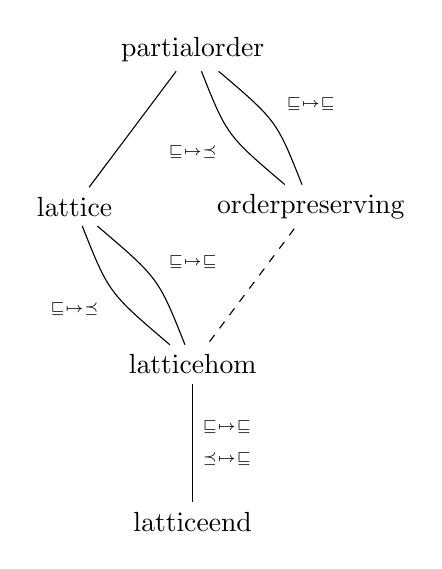
\begin{tikzpicture}
  \node (o) at (0,0) {\isa{partial{\isacharunderscore}order}};
  \node (oh) at (1.5,-2) {\isa{order{\isacharunderscore}preserving}};
  \node (oh1) at (1.5,-0.7) {$\scriptscriptstyle \sqsubseteq \mapsto \sqsubseteq$};
  \node (oh2) at (0,-1.3) {$\scriptscriptstyle \sqsubseteq \mapsto \preceq$};
  \node (l) at (-1.5,-2) {\isa{lattice}};
  \node (lh) at (0,-4) {\isa{lattice{\isacharunderscore}hom}};
  \node (lh1) at (0,-2.7) {$\scriptscriptstyle \sqsubseteq \mapsto \sqsubseteq$};
  \node (lh2) at (-1.5,-3.3) {$\scriptscriptstyle \sqsubseteq \mapsto \preceq$};
  \node (le) at (0,-6) {\isa{lattice{\isacharunderscore}end}};
  \node (le1) at (0,-4.8)
    [anchor=west]{$\scriptscriptstyle \sqsubseteq \mapsto \sqsubseteq$};
  \node (le2) at (0,-5.2)
    [anchor=west]{$\scriptscriptstyle \preceq \mapsto \sqsubseteq$};
  \draw (o) -- (l);
  \draw[dashed] (oh) -- (lh);
  \draw (lh) -- (le);
  \draw (o) .. controls (oh1.south west) .. (oh);
  \draw (o) .. controls (oh2.north east) .. (oh);
  \draw (l) .. controls (lh1.south west) .. (lh);
  \draw (l) .. controls (lh2.north east) .. (lh);
\end{tikzpicture}
\end{center}
\hrule
\caption{Hierarchy of Homomorphism Locales.}
\label{fig:hom}
\end{figure}%
\end{isamarkuptext}%
\isamarkuptrue%
%
\begin{isamarkuptext}%
It can be shown easily that a lattice homomorphism is order
  preserving.  As the final example of this section, a locale
  interpretation is used to assert this.%
\end{isamarkuptext}%
\isamarkuptrue%
\ \ \isacommand{sublocale}\isamarkupfalse%
\ lattice{\isacharunderscore}hom\ {\isasymsubseteq}\ order{\isacharunderscore}preserving%
\isadelimproof
\ %
\endisadelimproof
%
\isatagproof
\isacommand{proof}\isamarkupfalse%
\ unfold{\isacharunderscore}locales\isanewline
\ \ \ \ \isacommand{fix}\isamarkupfalse%
\ x\ y\isanewline
\ \ \ \ \isacommand{assume}\isamarkupfalse%
\ {\isachardoublequoteopen}x\ {\isasymsqsubseteq}\ y{\isachardoublequoteclose}\isanewline
\ \ \ \ \isacommand{then}\isamarkupfalse%
\ \isacommand{have}\isamarkupfalse%
\ {\isachardoublequoteopen}y\ {\isacharequal}\ {\isacharparenleft}x\ {\isasymsqunion}\ y{\isacharparenright}{\isachardoublequoteclose}\ \isacommand{by}\isamarkupfalse%
\ {\isacharparenleft}simp\ add{\isacharcolon}\ join{\isacharunderscore}connection{\isacharparenright}\isanewline
\ \ \ \ \isacommand{then}\isamarkupfalse%
\ \isacommand{have}\isamarkupfalse%
\ {\isachardoublequoteopen}{\isasymphi}\ y\ {\isacharequal}\ {\isacharparenleft}{\isasymphi}\ x\ {\isasymsqunion}{\isacharprime}\ {\isasymphi}\ y{\isacharparenright}{\isachardoublequoteclose}\ \isacommand{by}\isamarkupfalse%
\ {\isacharparenleft}simp\ add{\isacharcolon}\ hom{\isacharunderscore}join\ {\isacharbrackleft}symmetric{\isacharbrackright}{\isacharparenright}\isanewline
\ \ \ \ \isacommand{then}\isamarkupfalse%
\ \isacommand{show}\isamarkupfalse%
\ {\isachardoublequoteopen}{\isasymphi}\ x\ {\isasympreceq}\ {\isasymphi}\ y{\isachardoublequoteclose}\ \isacommand{by}\isamarkupfalse%
\ {\isacharparenleft}simp\ add{\isacharcolon}\ lat{\isacharprime}{\isachardot}join{\isacharunderscore}connection{\isacharparenright}\isanewline
\ \ \isacommand{qed}\isamarkupfalse%
%
\endisatagproof
{\isafoldproof}%
%
\isadelimproof
%
\endisadelimproof
%
\begin{isamarkuptext}%
Theorems and other declarations --- syntax, in particular ---
  from the locale \isa{order{\isacharunderscore}preserving} are now active in \isa{lattice{\isacharunderscore}hom}, for example

  \isa{lat{\isacharprime}{\isachardot}less{\isacharunderscore}le{\isacharunderscore}trans}:
  \isa{{\isasymlbrakk}{\isacharquery}x\ {\isasymprec}\ {\isacharquery}y{\isacharsemicolon}\ {\isacharquery}y\ {\isasympreceq}\ {\isacharquery}z{\isasymrbrakk}\ {\isasymLongrightarrow}\ {\isacharquery}x\ {\isasymprec}\ {\isacharquery}z}%
\end{isamarkuptext}%
\isamarkuptrue%
%
\isamarkupsection{Further Reading%
}
\isamarkuptrue%
%
\begin{isamarkuptext}%
More information on locales and their interpretation is
  available.  For the locale hierarchy of import and interpretation
  dependencies see \cite{Ballarin2006a}; interpretations in theories
  and proofs are covered in \cite{Ballarin2006b}.  In the latter, we
  show how interpretation in proofs enables to reason about families
  of algebraic structures, which cannot be expressed with locales
  directly.

  Haftmann and Wenzel \cite{HaftmannWenzel2007} overcome a restriction
  of axiomatic type classes through a combination with locale
  interpretation.  The result is a Haskell-style class system with a
  facility to generate Haskell code.  Classes are sufficient for
  simple specifications with a single type parameter.  The locales for
  orders and lattices presented in this tutorial fall into this
  category.  Order preserving maps, homomorphisms and vector spaces,
  on the other hand, do not.

  The original work of Kamm\"uller on locales \cite{KammullerEtAl1999}
  may be of interest from a historical perspective.  The mathematical
  background on orders and lattices is taken from Jacobson's textbook
  on algebra \cite[Chapter~8]{Jacobson1985}.%
\end{isamarkuptext}%
\isamarkuptrue%
%
\begin{isamarkuptext}%
\begin{table}
\hrule
\vspace{2ex}
\begin{center}
\begin{tabular}{l>$c<$l}
  \multicolumn{3}{l}{Miscellaneous} \\

  \textit{attr-name} & ::=
  & \textit{name} $|$ \textit{attribute} $|$
    \textit{name} \textit{attribute} \\[2ex]

  \multicolumn{3}{l}{Context Elements} \\

  \textit{fixes} & ::=
  & \textit{name} [ ``\textbf{::}'' \textit{type} ]
    [ ``\textbf{(}'' \textbf{structure} ``\textbf{)}'' $|$
    \textit{mixfix} ] \\
\begin{comment}
  \textit{constrains} & ::=
  & \textit{name} ``\textbf{::}'' \textit{type} \\
\end{comment}
  \textit{assumes} & ::=
  & [ \textit{attr-name} ``\textbf{:}'' ] \textit{proposition} \\
\begin{comment}
  \textit{defines} & ::=
  & [ \textit{attr-name} ``\textbf{:}'' ] \textit{proposition} \\
  \textit{notes} & ::=
  & [ \textit{attr-name} ``\textbf{=}'' ]
    ( \textit{qualified-name} [ \textit{attribute} ] )$^+$ \\
\end{comment}

  \textit{element} & ::=
  & \textbf{fixes} \textit{fixes} ( \textbf{and} \textit{fixes} )$^*$ \\
\begin{comment}
  & |
  & \textbf{constrains} \textit{constrains}
    ( \textbf{and} \textit{constrains} )$^*$ \\
\end{comment}
  & |
  & \textbf{assumes} \textit{assumes} ( \textbf{and} \textit{assumes} )$^*$ \\[2ex]
%\begin{comment}
%  & |
%  & \textbf{defines} \textit{defines} ( \textbf{and} \textit{defines} )$^*$ \\
%  & |
%  & \textbf{notes} \textit{notes} ( \textbf{and} \textit{notes} )$^*$ \\
%\end{comment}

  \multicolumn{3}{l}{Locale Expressions} \\

  \textit{rename} & ::=
  & \textit{name} [ \textit{mixfix} ] $|$ ``\textbf{\_}'' \\
  \textit{expr}  & ::= 
  & \textit{renamed-expr} ( ``\textbf{+}'' \textit{renamed-expr} )$^*$ \\
  \textit{renamed-expr} & ::=
  & ( \textit{qualified-name} $|$
    ``\textbf{(}'' \textit{expr} ``\textbf{)}'' ) \textit{rename}$^*$ \\[2ex]

  \multicolumn{3}{l}{Declaration of Locales} \\

  \textit{locale} & ::=
  & \textit{element}$^+$ \\
  & | & \textit{locale-expr} [ ``\textbf{+}'' \textit{element}$^+$ ] \\
  \textit{toplevel} & ::=
  & \textbf{locale} \textit{name} [ ``\textbf{=}''
    \textit{locale} ] \\[2ex]

  \multicolumn{3}{l}{Interpretation} \\

  \textit{equation} & ::= & [ \textit{attr-name} ``\textbf{:}'' ]
    \textit{prop} \\
  \textit{insts} & ::= & [ ``\textbf{[}'' \textit{term}$^+$
    ``\textbf{]}'' ] \\
  & & [ \textbf{where} \textit{equation} ( \textbf{and}
    \textit{equation} )$^*$ ] \\
  \textit{toplevel} & ::=
  & \textbf{interpretation} \textit{name} ( ``$<$'' $|$
    ``$\subseteq$'' ) \textit{expr} \textit{proof} \\
  & |
  & \textbf{interpretation} [ \textit{attr-name} ``\textbf{:}'' ]
    \textit{expr} \textit{insts} \textit{proof} \\
  & |
  & \textbf{interpret} [ \textit{attr-name} ``\textbf{:}'' ]
    \textit{expr} \textit{insts} \textit{proof} \\[2ex]

  \multicolumn{3}{l}{Diagnostics} \\

  \textit{toplevel} & ::=
  & \textbf{print\_locale} [ ``\textbf{!}'' ] \textit{locale} \\
  & | & \textbf{print\_locales} 
\end{tabular}
\end{center}
\hrule
\caption{Syntax of Locale Commands.}
\label{tab:commands}
\end{table}%
\end{isamarkuptext}%
\isamarkuptrue%
%
\begin{isamarkuptext}%
\textbf{Acknowledgements.}  Alexander Krauss, Tobias Nipkow,
  Christian Sternagel and Makarius Wenzel have made useful comments on
  a draft of this document.%
\end{isamarkuptext}%
\isamarkuptrue%
%
\isadelimtheory
%
\endisadelimtheory
%
\isatagtheory
\isacommand{end}\isamarkupfalse%
%
\endisatagtheory
{\isafoldtheory}%
%
\isadelimtheory
%
\endisadelimtheory
\isanewline
\end{isabellebody}%
%%% Local Variables:
%%% mode: latex
%%% TeX-master: "root"
%%% End:
